\subsection{Results} \label{subsec:results_linear_regression}

This \href{https://github.com/am-kaiser/CompSci-Project-1/blob/main/regression_analysis/examples/linear_regression_analysis.ipynb}{jupyter notebook} consists of examples to apply different regression techniques. It also consists of widgets where the precalculated statistical performance of different regression methods can be viewed for over $10^5$ parameter combinations. The data for these experiments is included in the repository. At the end of the jupyter notebook, one can find code that will allow for simulating more parameter combinations if needed. This will overwrite the existing data and also would take a significant time to run. For $10^5$ parameter combinations, it took us about $2$ hours to obtain the data.

\subsubsection{Terminology of symbols and variable names}
Here, we list the names of the variables that are the options in the widgets of the jupyter notebook. The corresponding symbols if applicable are also shown. These symbols relate the variable names to their corresponding mathematical notation used in this report. The general template is the following \\
\\
Symbol: variable name → explanation \\
\\
The list of widget variables are:
\begin{itemize}
    \item $p:$  polynomial order → the order of 2D polynomial used for fitting
    \item $var:$  noise\_var → the variance of the zero mean Gaussian noise added to the Franke data
    \item $r:$  ratio → testing ratio. For example, if the ratio is 0.1 then the test set comprises 10 percent of the dataset.
    \item $n:$  num → the number of points taken along each direction of the input vector. If num = 20, then the total number of data points is 20*20 = 400
    \item stat → Displays the chosen statistic
    \begin{itemize}
        \item $MSE_{train}:$ training MSE
        \item $MSE_{test}:$ testing MSE
        \item ${R^2_{train}}:$ training R2 score
        \item ${R^2_{test}}:$ testing R2 score
        \item $bias_{test}:$ bias in test data
        \item $var_{test}:$ variance in test prediction
    \end{itemize}
    \item method → to choose the regression type
    \begin{itemize}
        \item direct solution and stochastic gradient descent solution available
        \begin{itemize}
            \item OLS
            \item OLS with bootstrap resampling
            \item OLS with cross-validation resampling
            \item Ridge
            \item Ridge with bootstrap resampling
            \item Ridge with cross-validation resampling
        \end{itemize}
        \item direct Solution only (using scikit learn)
        \begin{itemize}
            \item Lasso
            \item Lasso with bootstrap resampling
            \item Lasso with cross-validation resampling
        \end{itemize}
    \end{itemize}
    \item $n_b:$  n\_boot → number of times bootstrap sampling is performed in the bootstrap method. Changing this for methods that don't involve bootstrap sampling will not have any effect
    \item $k_f:$  k\_fold → number of folds in the cross-validation method. Changing this for methods that don't involve cross-validation will not have any effect
    \item $\lambda_r:$  ridge\_lambda → regularisation parameter for ridge regression
    \item $\lambda_l:$ lasso\_lambda → regularisation parameter for lasso regression
    \item $\eta:$ learn\_rates → parameter that controls the descent jump size in gradient descent methods
    \item $n_e:$ epoch → parameter that controls the number of times the algorithm works through the entire dataset in gradient descent methods
    \item $n_{batch}:$ number of batches → parameter that controls the mini-batch size in gradient descent methods
\end{itemize}

Here, we present selected results of linear regression that we find particularly interesting. 

\subsubsection{Ordinary Least Squares (OLS)}

Foremost, we look at the $MSE_{train}$ of OLS (see figure \ref{fig:ols1}). We see that the $MSE_{train}$ reduces as the model complexity or polynomial order($p$) increases. In other words, with increasing complexity, our model becomes more flexible. As the input data is an exponential function that can be expressed as a series of polynomials, increasing the terms in the fitted polynomial should decrease the $MSE_{train}$. We also see that for large values of test ratio, i.e. $r = 0.4$, and low number of data points, $n = 100$, which amounts to about $60$ data points in the training set, the $MSE_{train}$ is significantly lower for high $p$.

\begin{figure}[htb]
\centering
\begin{subfigure}{.5\textwidth}
  \centering
  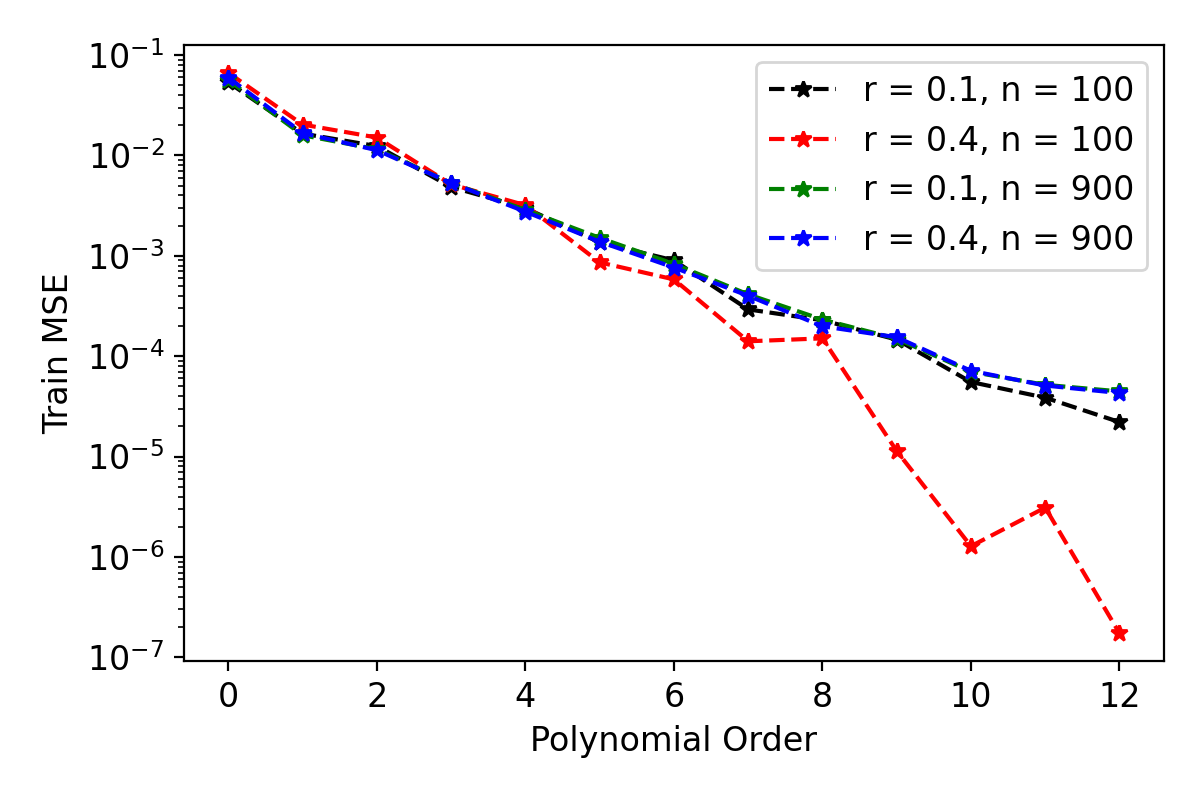
\includegraphics[width=.9\linewidth]{Images/ols2.png}
  \caption{}
  \label{fig:ols1}
\end{subfigure}%
\begin{subfigure}{.5\textwidth}
  \centering
  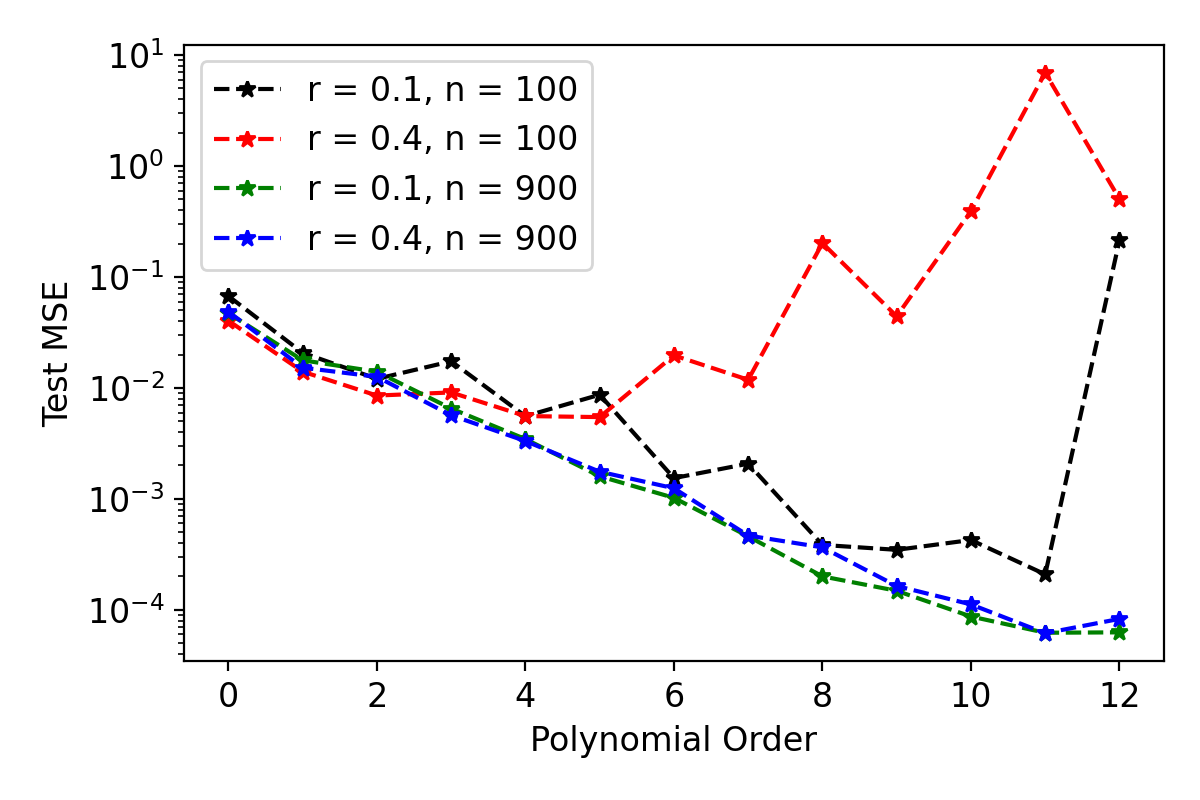
\includegraphics[width=.9\linewidth]{Images/ols1.png}
  \caption{}
  \label{fig:ols2}
\end{subfigure}
\begin{subfigure}{.5\textwidth}
  \centering
  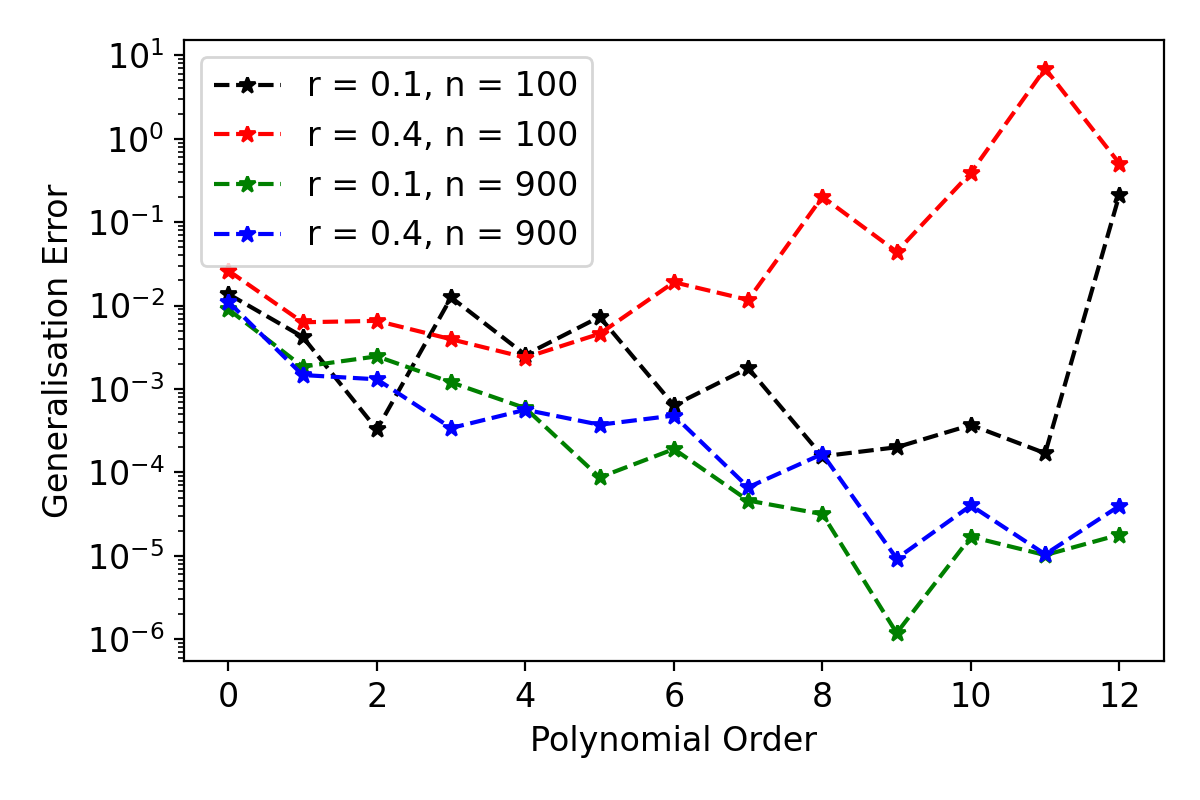
\includegraphics[width=.9\linewidth]{Images/ols3.png}
  \caption{}
  \label{fig:ols3}
\end{subfigure}
\begin{subfigure}{.45\textwidth}
  \centering
  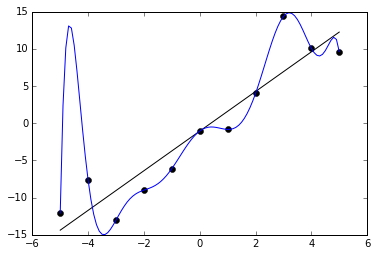
\includegraphics[width=.9\linewidth]{Images/Overfitted_Data.png}
  \caption{}
  \label{fig:overfit}
\end{subfigure}
\caption{OLS for noiseless Franke data: (a) $MSE_{train}$, (b) $MSE_{test}$ and (c) Generalization error plotted as functions of model complexity. (d) Schematic describing overfitting of data due to higher model complexity (Source: Ghiles, Wikipedia). }
\label{fig:OLS1}
\end{figure}

Now, if we shift attention to the $MSE_{test}$, we see that for r=0.4, n=100, the generalization is poor (see figure \ref{fig:ols2}). This is the result of overfitting. This also happens for r=0.1, n=100 albeit not as strongly. This reveals that even for low values of $MSE_{train}$, the model can perform poorly. We recognize that if the number of datapoints is higher in the training set, then there is no overfitting. This is also evident by looking at the generalization error(see figure \ref{fig:ols3}). The model 'sees' more variety of data during the training phase which prevents it from overfitting. Provided we don't overfit, the $MSE_{test}$ reduces as p  increases. It should be noted that irrespective of the number of data points used for training, there exist p's where we will experience overfitting. The figure \ref{fig:overfit} shows a 1D polynomial with order equal to the number of points which will perform much worse than a linear polynomial for unseen data. If $n_{train}$ is the number of training data points then to prevent overfitting in many situations, we need $n_{train} >> p$. 
\newline
\newline
Next, we see that the introduction of noise into the dataset increases $MSE_{train}$ (see figure \ref{fig:ols4}). We also see that introducing noise affects the $MSE_{test}$ of a dataset with a larger number of points significantly when model complexity is high (see figure \ref{fig:ols5}). $MSE_{test}$ decreases initially with model complexity but later plateaus. This portrays that the higher degree of freedom, introduced by additional polynomial terms, doesn't sufficiently capture the noise. When the model complexity is low, the prediction is unaffected by the presence of noise. 
\newline\newline
\begin{figure}[htb]
\centering
\begin{subfigure}{.5\textwidth}
  \centering
  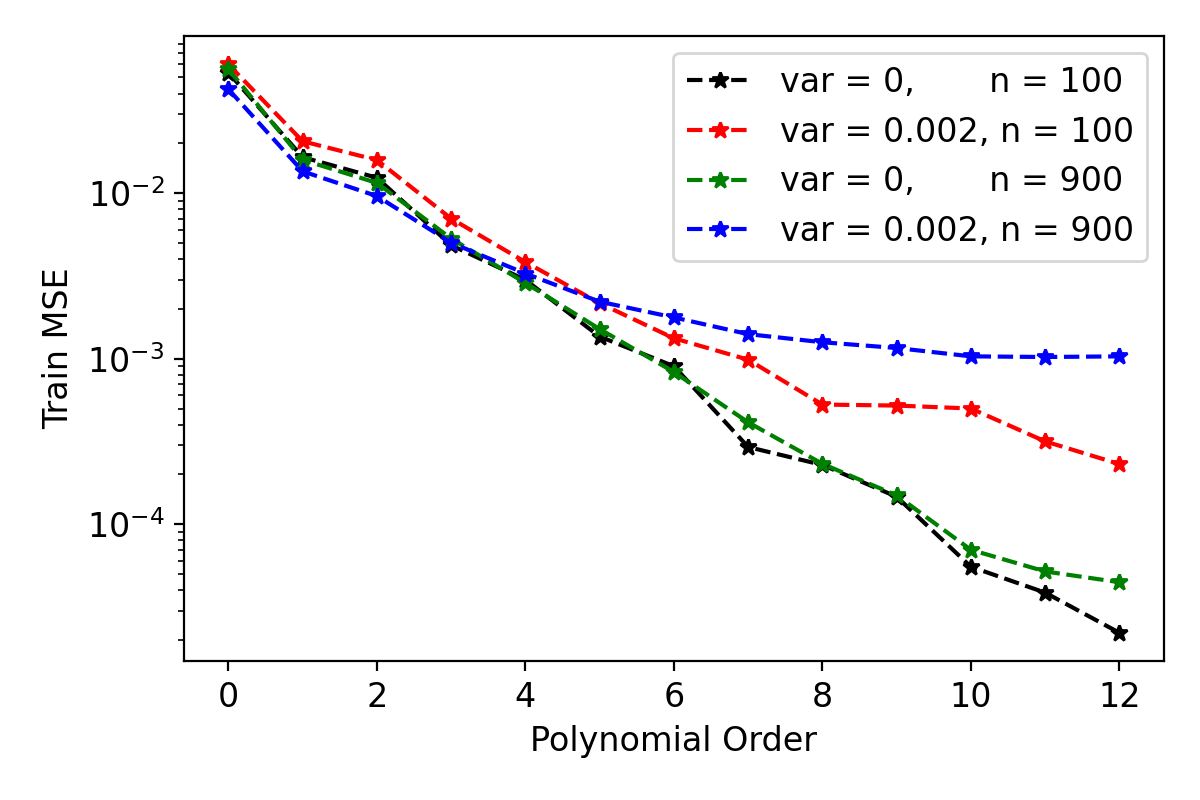
\includegraphics[width=.9\linewidth]{Images/ols5.png}
  \caption{}
  \label{fig:ols4}
\end{subfigure}%
\begin{subfigure}{.5\textwidth}
  \centering
  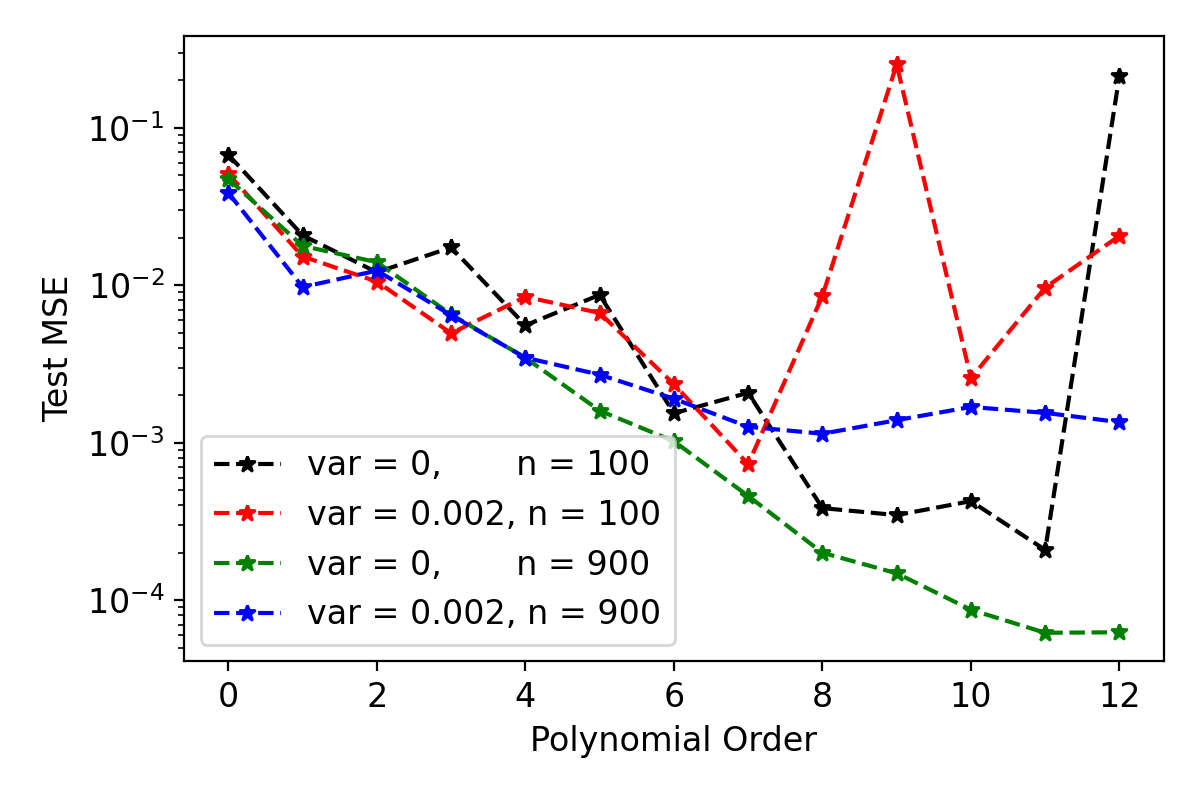
\includegraphics[width=.9\linewidth]{Images/ols4.png}
  \caption{}
  \label{fig:ols5}
\end{subfigure}
\caption{OLS for $r=0.1$ and $n=900$: (a) $MSE_{train}$ and (b) $MSE_{test}$ plotted as functions of model complexity}
\label{fig:OLS2}
\end{figure}

\begin{figure}[htb]
\centering
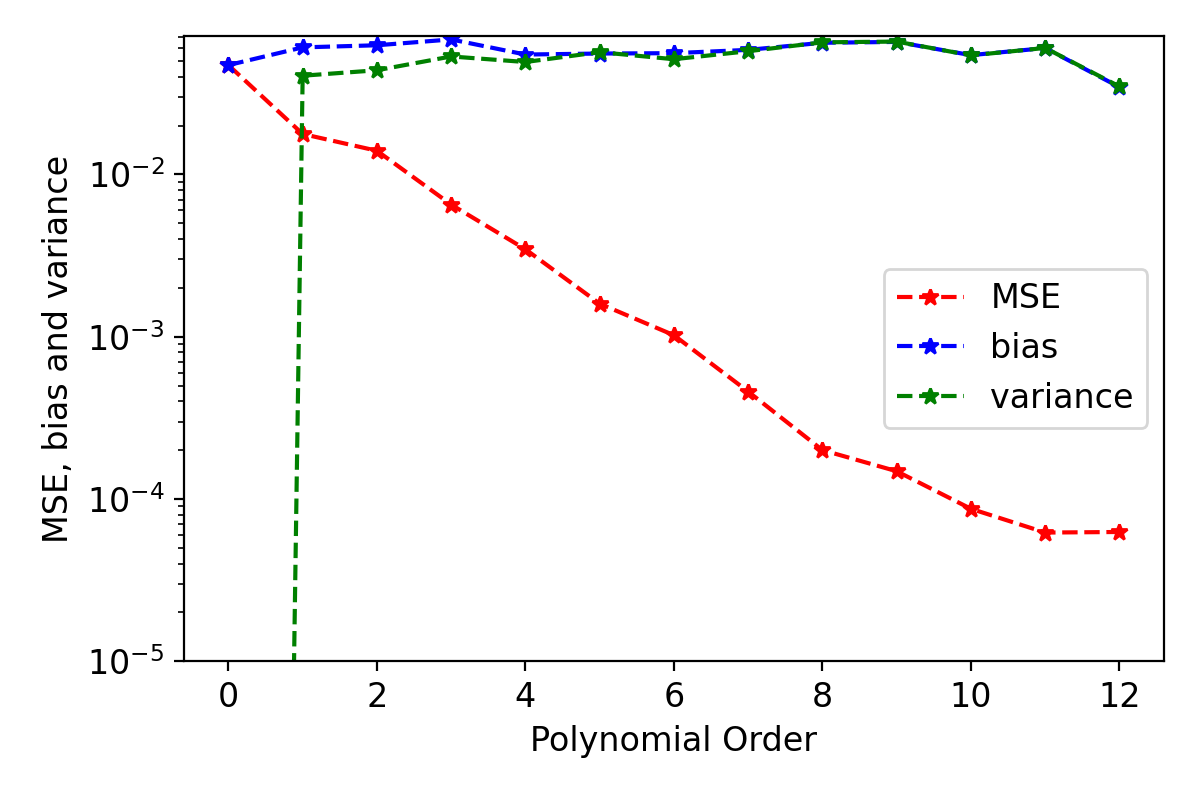
\includegraphics[width=.7\linewidth]{Images/ols7.png}
\caption{OLS for $r=0.1$, $var=0$ and $n=900$. Bias and variance plotted as functions of model complexity}
\label{fig:OLS3}
\end{figure}

If we now look at the bias and variance, they are both roughly constant as the model complexity increases (see figure \ref{fig:OLS3}). This might be a discrepancy in our calculation and it prevents us from understanding the bias-variance tradeoff. This behavior is observed even when other parameters are changed. As variance measures, the spread of our prediction, and the plots show that our model always has a finite spread. As bias is a measure of the mean deviation of our prediction from the truth, the constant values raise questions on our calculations. We know that parameters like $r$, $var$, $p$ and $n$ have an impact on the $MSE_{test}$, but as the bias seems to be roughly the same then that shows that irrespective of the parameters, our model has approximately the same mean value of the predicted output. Either our model is capturing the mean well almost always or our calculations of bias and variance are incorrect.

\subsubsection{Ridge and lasso Regression}
In ridge regression, we use the $L_2$ norm of the parameter vector $\boldsymbol \beta$ as a penalty term. As we are not tuning the size of the elements of the design matrix, the interrelations between the different columns should remain the same. This is the case when the design matrix is orthogonal. As we use polynomials as basis functions, the columns of the design matrix are likely to be independent. They will not be independent if there is a correlation between $x_{i1}$ and $x_{i2}$ which is not true in our dataset. So, the parameters in ridge regression would be rescaled by a factor of $\frac{1}{1+\lambda_r}$ compared to the OLS parameters \cite{mehta2019high}. However, since that there might be errors in calculating the pseudoinverse, the scaling might not always be by the factor of $\frac{1}{1+\lambda_r}$. So, not all parameters are scaled the same. This would deviate the predictions from that of the OLS. We can see this in the figure \ref{fig:ridge7} and \ref{fig:ridge7b} where the regularisation parameter affects both the training and prediction phase. The training and testing error both worsen as $\lambda_r$ increases. The deviation from the OLS errors kicks in at a lower model complexity for higher values of  $\lambda_r$. For lower model complexity, the ridge regression performs similarly to OLS. But, as the complexity increases, ridge regression has a poorer prediction. It is unclear why this happens, but the most likely reason might be numeric underflow or overflow. 



\begin{figure}[htb]
\centering
\begin{subfigure}{.5\textwidth}
  \centering
  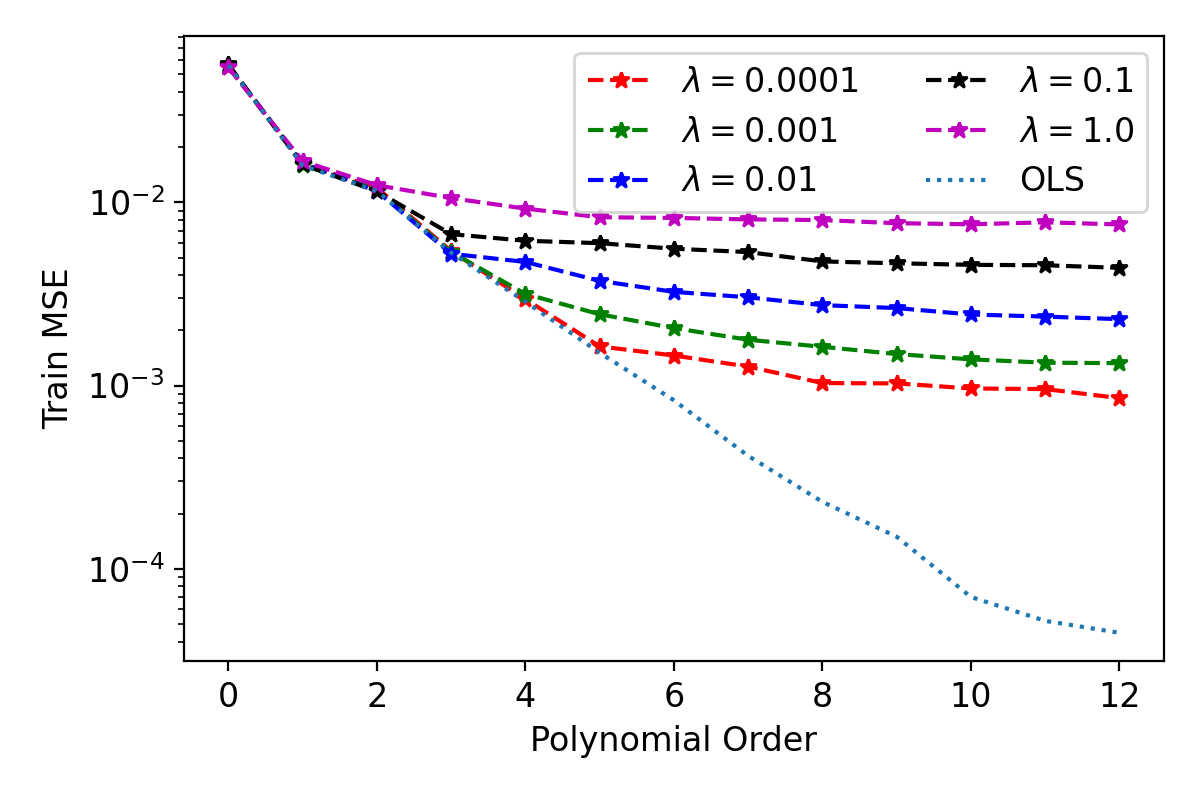
\includegraphics[width=.9\linewidth]{Images/ridge7b.png}
  \caption{}
  \label{fig:ridge7}
\end{subfigure}%
\begin{subfigure}{.5\textwidth}
  \centering
  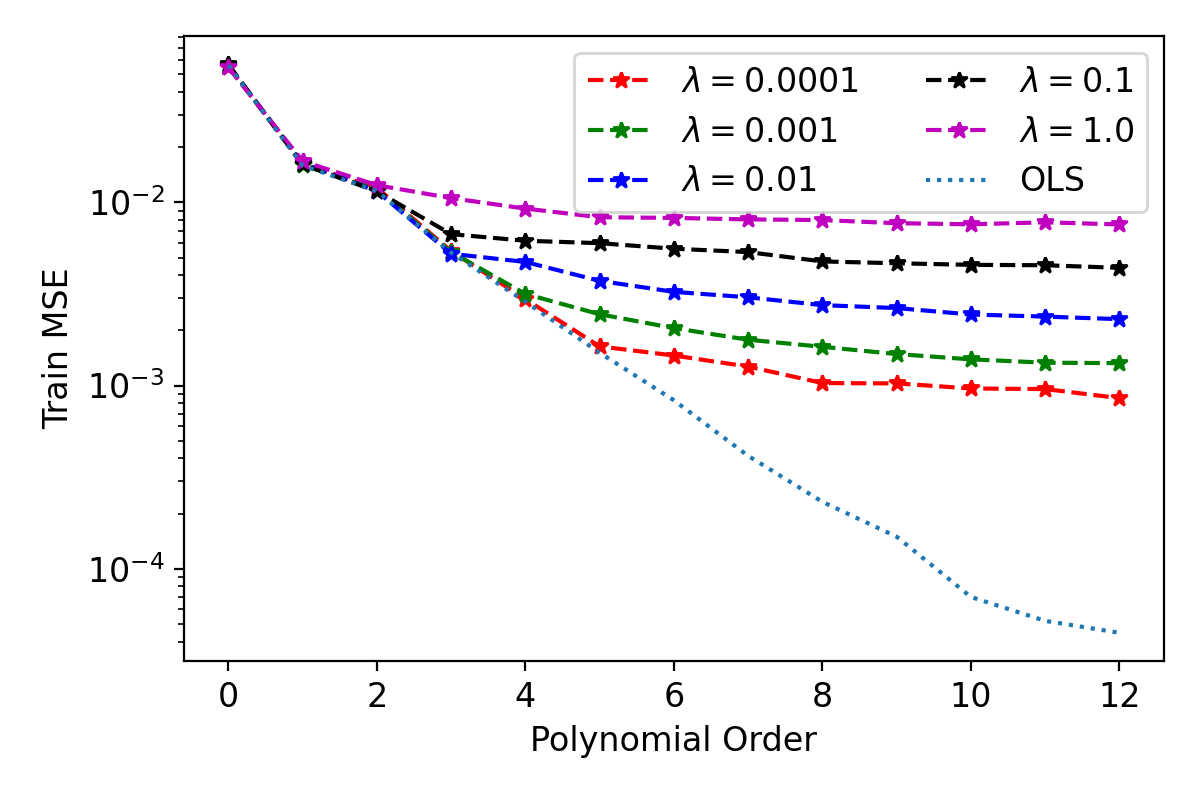
\includegraphics[width=.9\linewidth]{Images/ridge7b.png}
  \caption{}
  \label{fig:ridge7b}
\end{subfigure}
\caption{Ridge regression for $r=0.1$, $var=0$ and $n=900$: (a) $MSE_{train}$ and (b) $MSE_{test}$ plotted as functions of model complexity for different regularisation strength}
\label{fig:Ridge1}
\end{figure}

Meanwhile, in lasso regression, we use the $L_1$ norm of the parameter vector $\boldsymbol \beta$ as a penalty term. Visually, this is equivalent to optimizing the parameters until we hit the edges of a constraint hypercuboid. While, in ridge regression, we hit the surface of a constraint hyperellipsoid. See chapter 3 of \cite{friedman2001elements} for more details. This means that in lasso regression when the optimum parameters are reached, the components of some of the parameter vector $\boldsymbol \beta$ are 0. These features were not important enough in affecting the combined optimization of the least square error and the $L_1$ norm of the parameter vector $\boldsymbol \beta$. We see in the figure \ref{fig:lasso7} that both the training error and testing error worsen as the $\lambda_l$ increases. But, the performance is much worse than for ridge regression and is several orders of magnitude worse than OLS. As $\lambda_l$ increases, more components of $\boldsymbol \beta$ turn out to be 0. 


\begin{figure}[htb]
\centering
\begin{subfigure}{.5\textwidth}
  \centering
  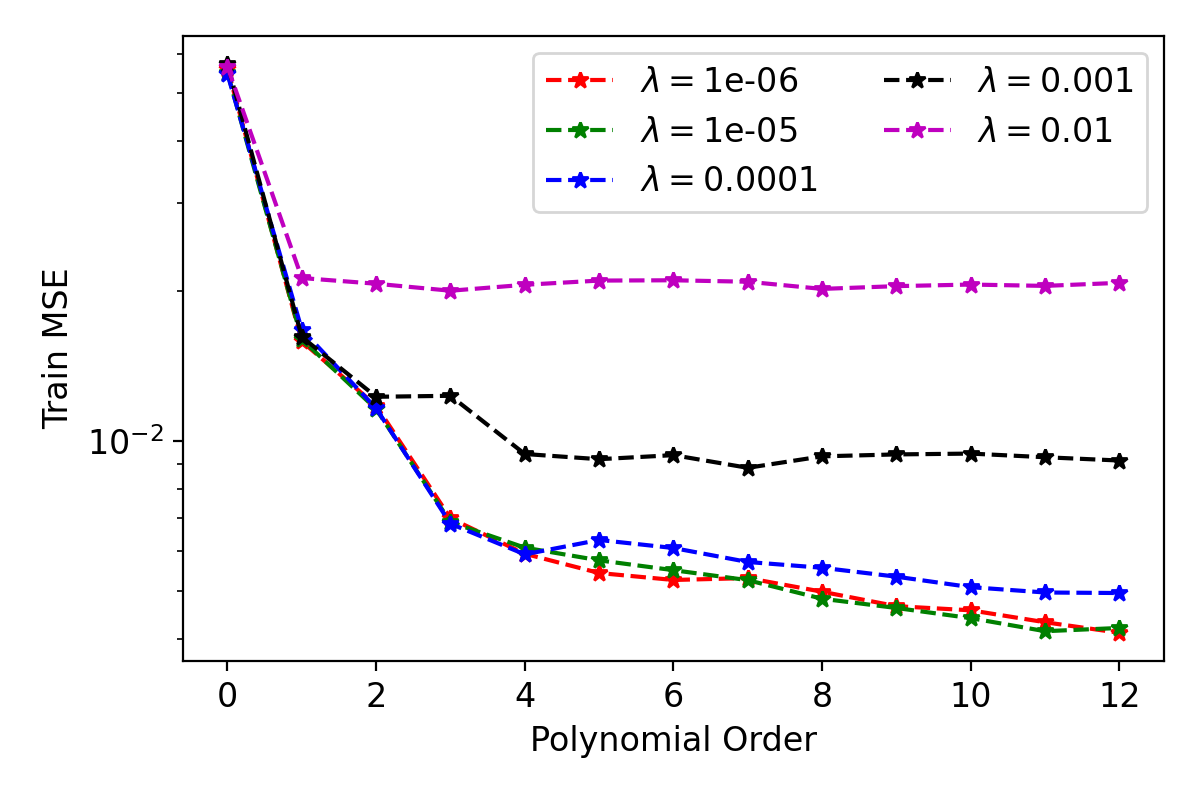
\includegraphics[width=.9\linewidth]{Images/lasso7b.png}
  \caption{}
  \label{fig:lasso7}
\end{subfigure}%
\begin{subfigure}{.5\textwidth}
  \centering
  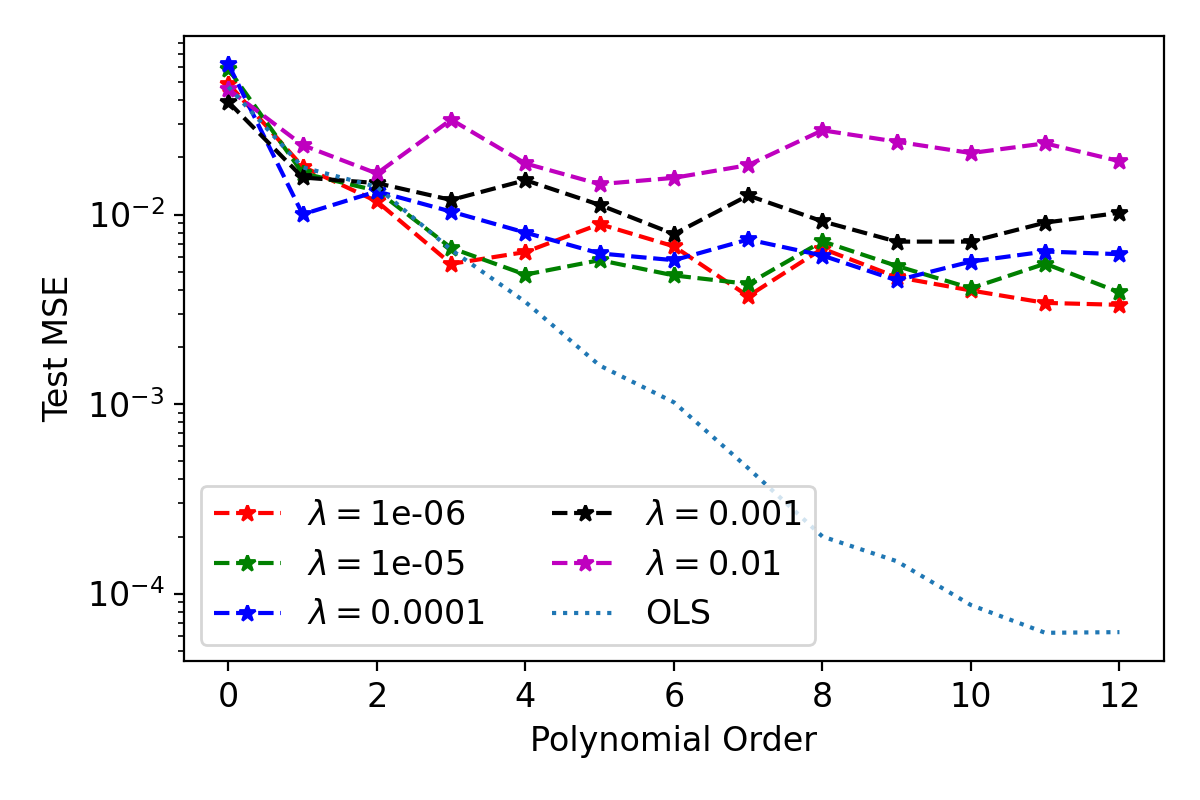
\includegraphics[width=.9\linewidth]{Images/lasso7.png}
  \caption{}
  \label{fig:lasso7b}
\end{subfigure}
\caption{lasso regression for $r=0.1$, $var=0$ and $n=900$: (a) $MSE_{train}$ and (b) $MSE_{test}$ plotted as functions of model complexity for different regularisation strength}
\label{fig:Lasso1}
\end{figure}

\begin{figure}[htb]
\centering
\begin{subfigure}{.5\textwidth}
  \centering
  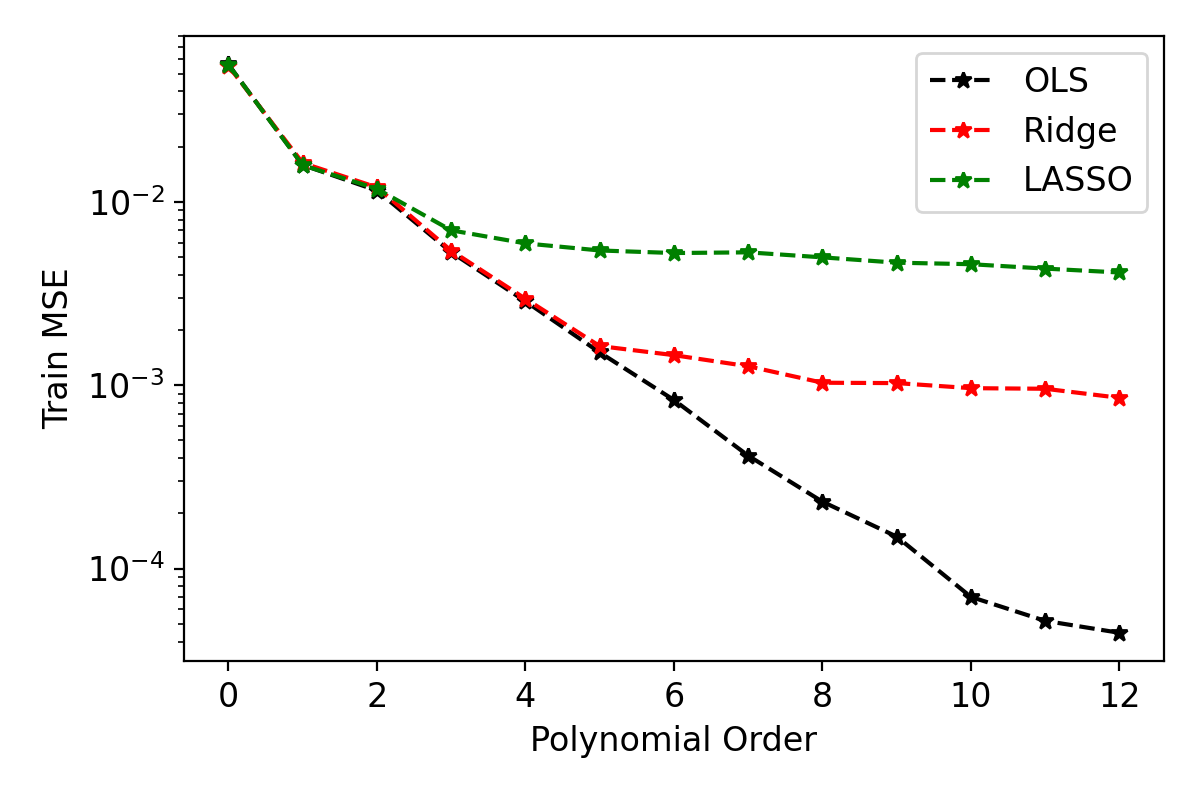
\includegraphics[width=.9\linewidth]{Images/orl2.png}
  \caption{}
  \label{fig:orl1}
\end{subfigure}%
\begin{subfigure}{.5\textwidth}
  \centering
  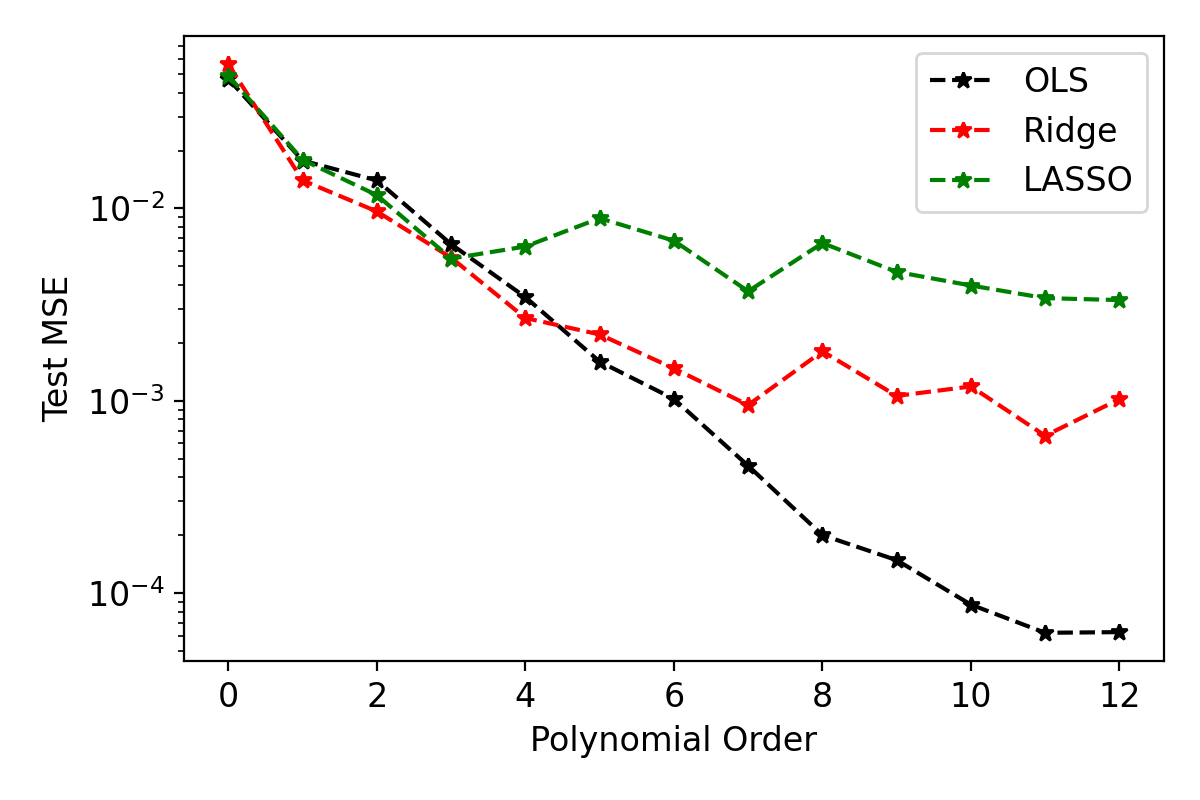
\includegraphics[width=.9\linewidth]{Images/orl1.png}
  \caption{}
  \label{fig:orl2}
\end{subfigure}
\begin{subfigure}{.5\textwidth}
  \centering
  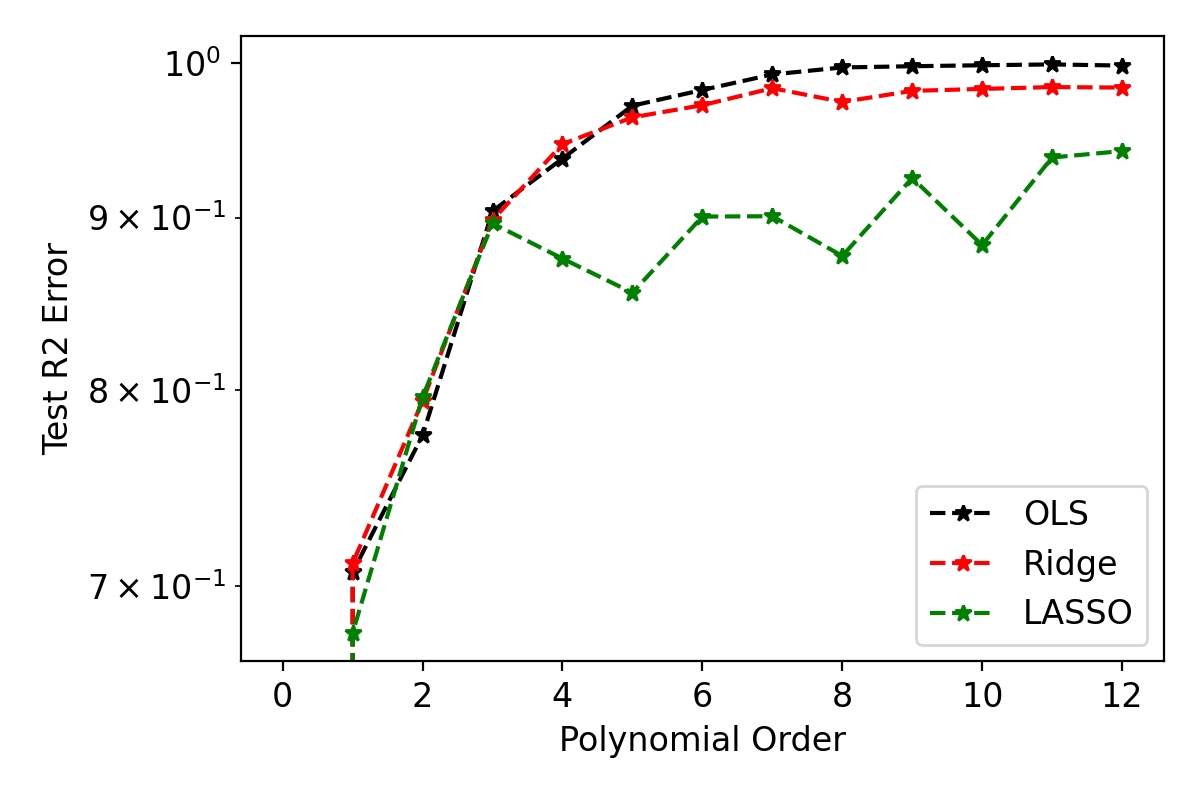
\includegraphics[width=.9\linewidth]{Images/orl3.png}
  \caption{}
  \label{fig:orl3}
\end{subfigure}
\caption{OLS, Ridge($\lambda_r = \num{1e-4}$) and lasso($\lambda_l = \num{1e-6}$) regression for $r=0.1$, $var=0$ and $n=900$: (a) $MSE_{train}$, (b) $MSE_{test}$ and (c) $R^2_{test}$ plotted as functions of model complexity}
\label{fig:ORL1}
\end{figure}

The figure \ref{fig:orl1} and \ref{fig:orl2} show the relative performance in training and testing for OLS, ridge, and lasso regression. Here, we show the best-case scenario for Ridge and lasso among the parameters screened by us. OLS outperforms ridge regression by an order of magnitude while it is 2 orders of magnitude better than lasso. This is explained by the fact that in OLS, the optimization involves lowering the squared error but in the other methods, there is an additional cost incurred for the size of components of parameter vectors. The figure \ref{fig:orl3} shows the $R^2_{test}$ error which is a measure of the variance captured by our model in relation to the actual variance. We see that as the model complexity increases, the $R^2_{test}$ tends to reach 1 for both OLS and ridge regression. While in lasso regression, the variance capture is much poorer. Certainly, the results here indicate that OLS performs much better than Ridge and lasso. Why would these two methods remain relevant? This is because there can be situations where the size of components of $\boldsymbol \beta$ can cause a numerical overflow. Additionally, shrinkage methods like Ridge and lasso reduce the prediction variability in many situations \cite{friedman2001elements}. 

\subsubsection{Regression with Bootstrap and Cross-validation}
\begin{figure}[ht]
\centering
\begin{subfigure}{.5\textwidth}
  \centering
  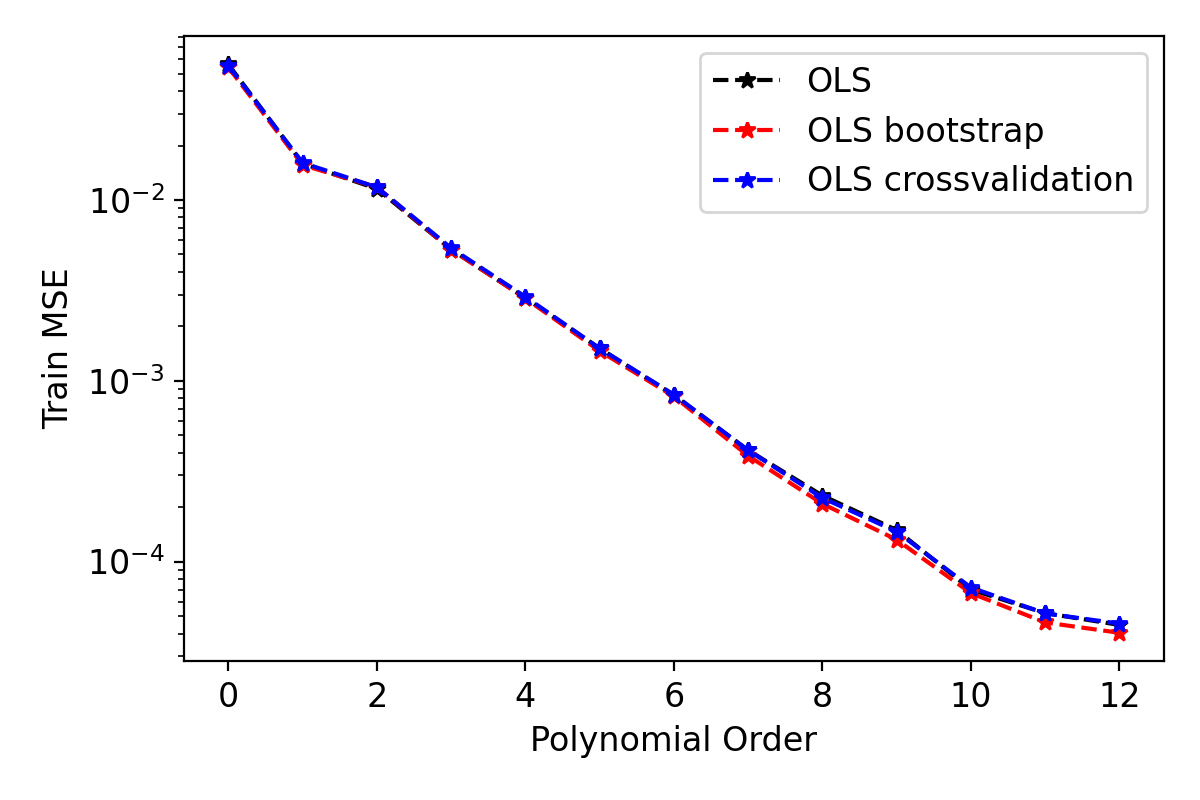
\includegraphics[width=.8\linewidth]{Images/ols9.png}
  \caption{}
  \label{fig:ols9}
\end{subfigure}%
\begin{subfigure}{.5\textwidth}
  \centering
  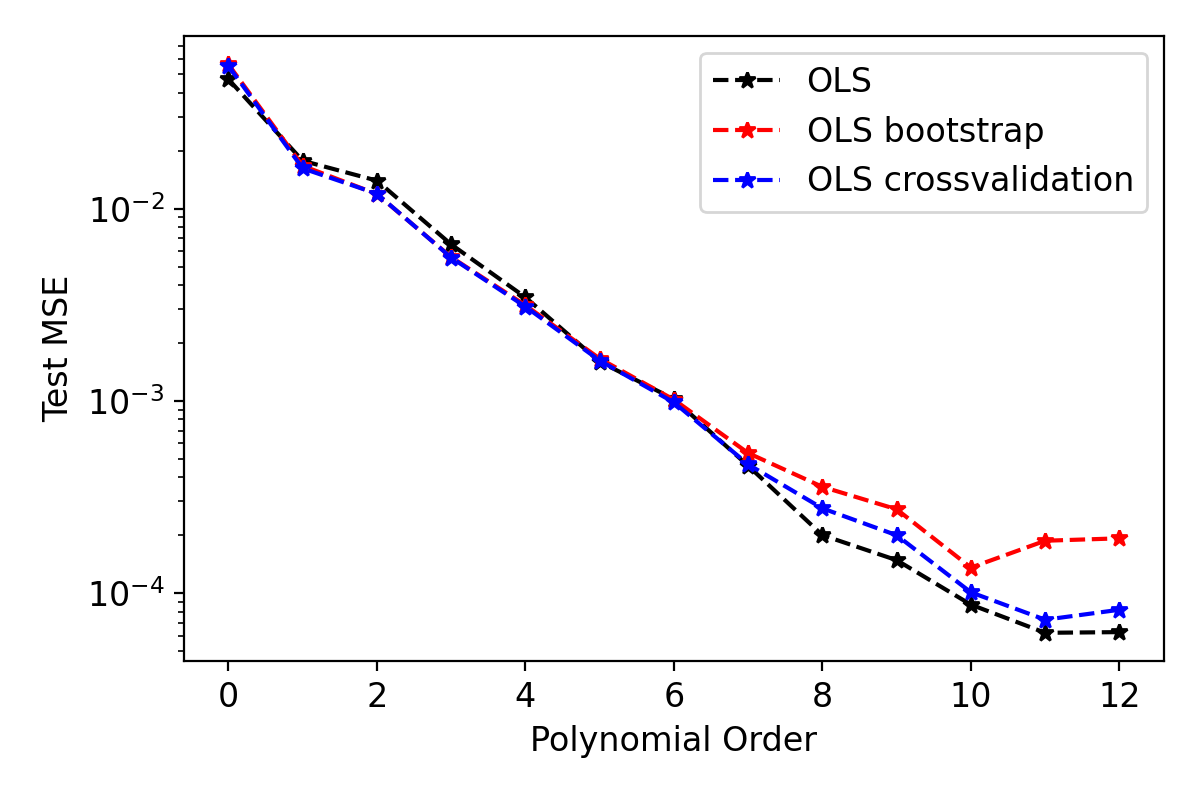
\includegraphics[width=.8\linewidth]{Images/ols8.png}
  \caption{}
  \label{fig:ols8}
\end{subfigure}
\begin{subfigure}{.5\textwidth}
  \centering
  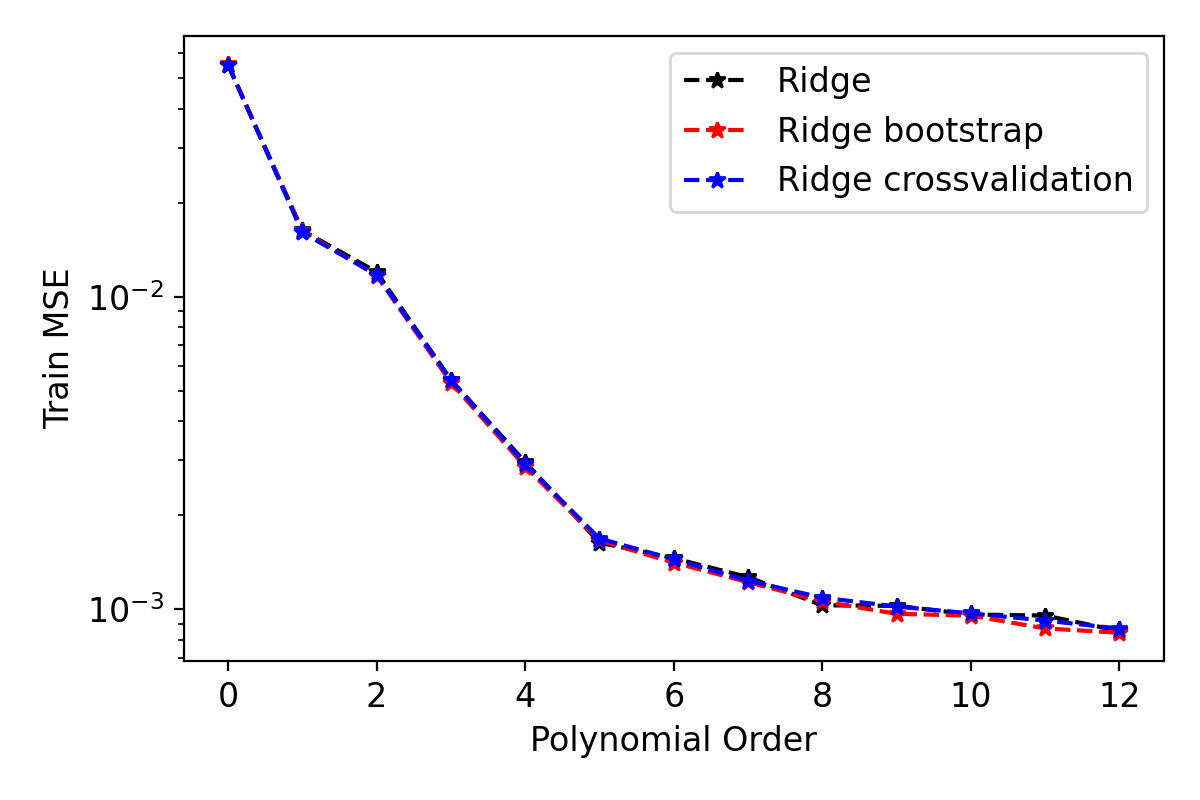
\includegraphics[width=.8\linewidth]{Images/ridge9.png}
  \caption{}
  \label{fig:ridge9}
\end{subfigure}%
\begin{subfigure}{.5\textwidth}
  \centering
  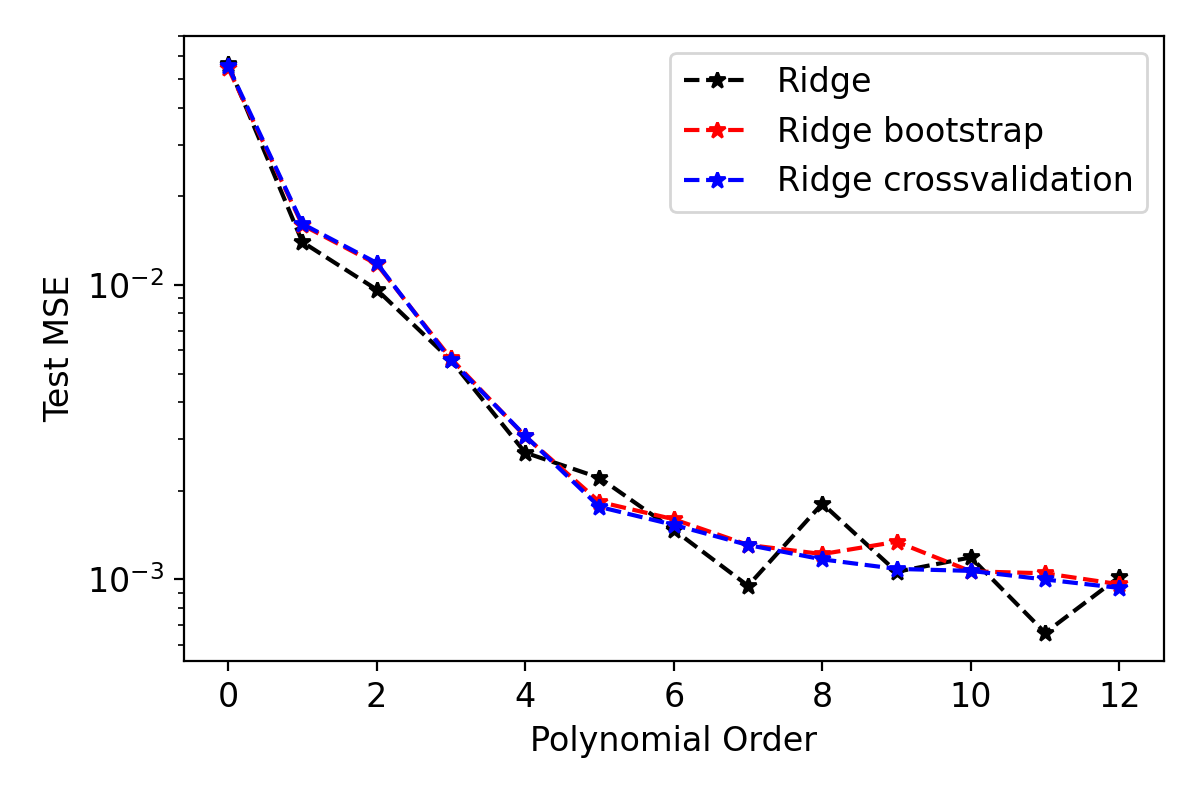
\includegraphics[width=.8\linewidth]{Images/ridge8.png}
  \caption{}
  \label{fig:ridge8}
\end{subfigure}
\begin{subfigure}{.5\textwidth}
  \centering
  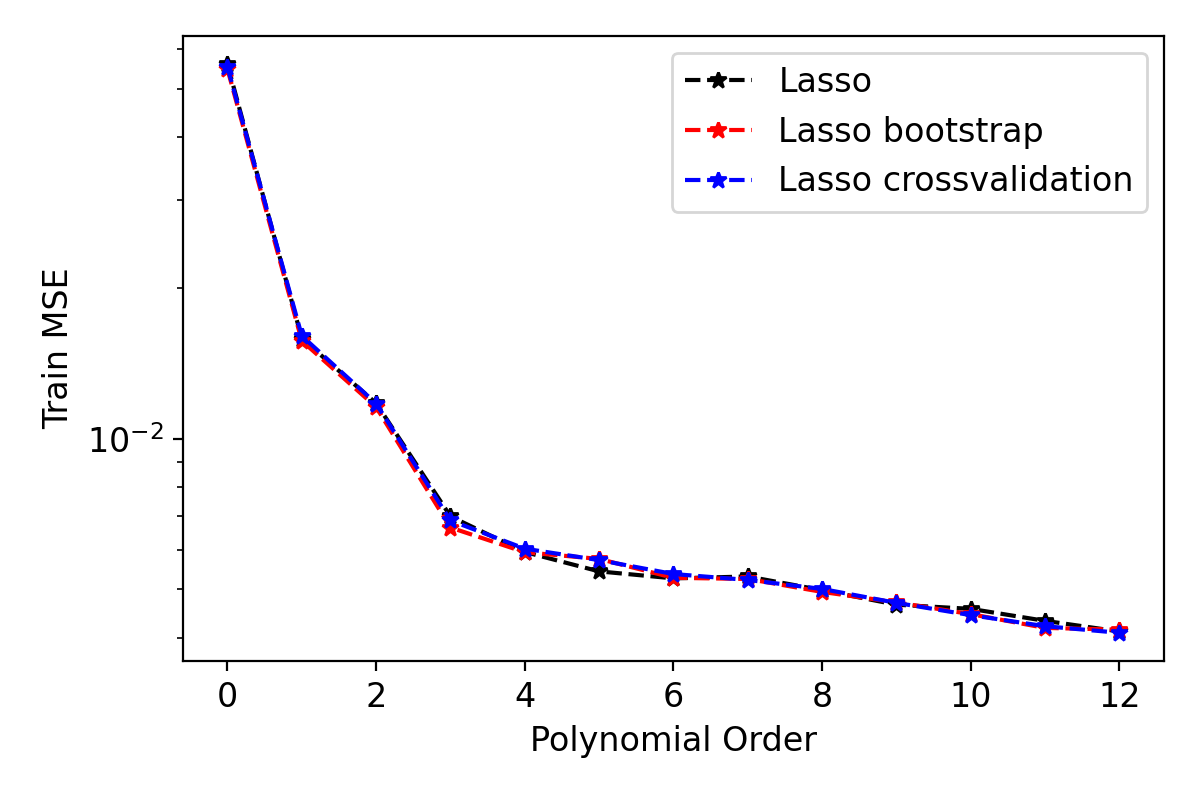
\includegraphics[width=.8\linewidth]{Images/lasso9.png}
  \caption{}
  \label{fig:lasso9}
\end{subfigure}%
\begin{subfigure}{.5\textwidth}
  \centering
  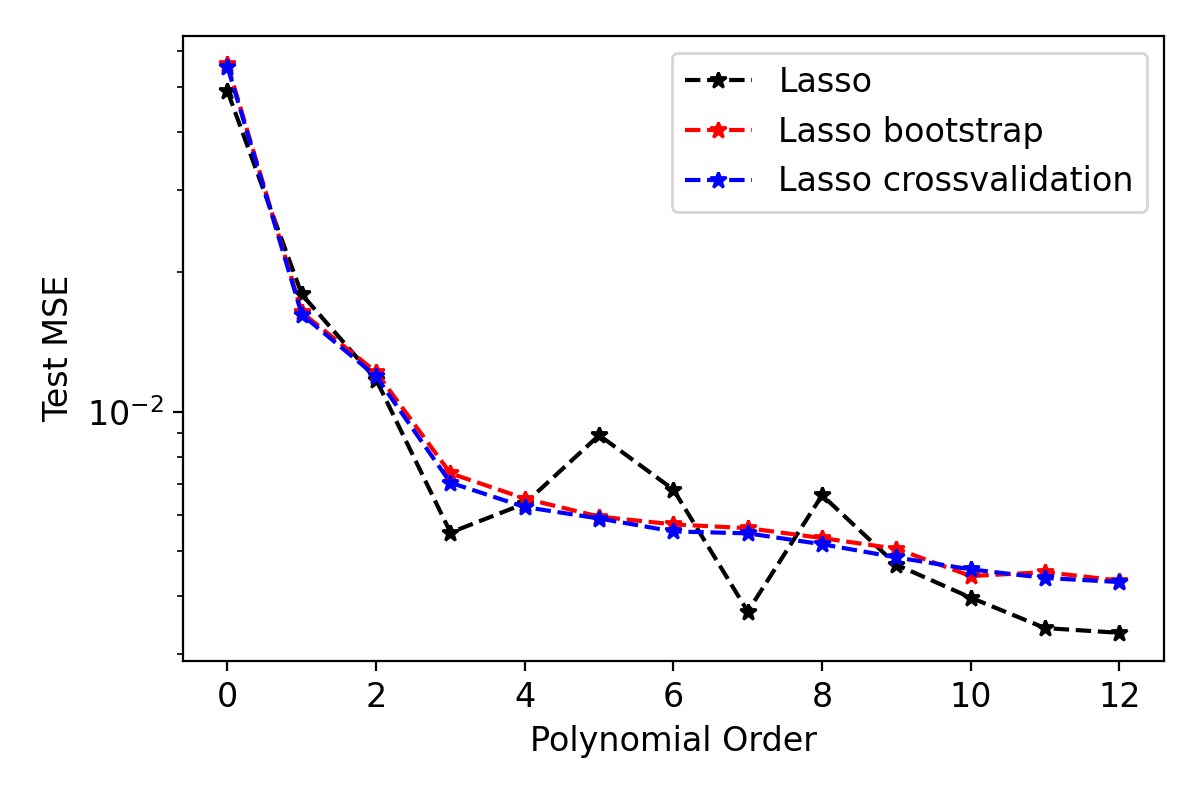
\includegraphics[width=.8\linewidth]{Images/lasso8.png}
  \caption{}
  \label{fig:lasso8}
\end{subfigure}
\caption{For $r=0.1$, $var=0$ and $n=900$: (a), (c), (e) $MSE_{train}$ and  (b), (d), (f) $MSE_{test}$ plotted as functions of model complexity}
\label{fig:OLS_resample}
\end{figure}


\begin{figure}[h!]
\centering
\begin{subfigure}{.5\textwidth}
  \centering
  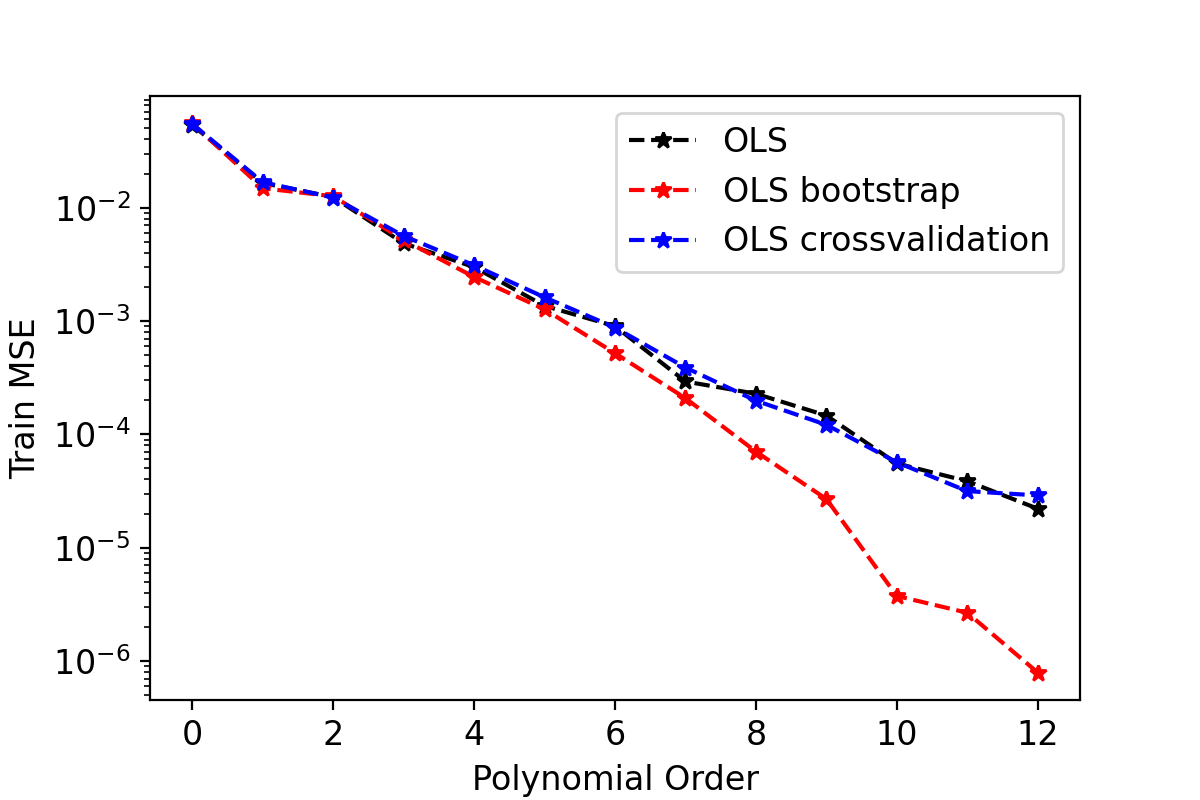
\includegraphics[width=.8\linewidth]{Images/ols15.png}
  \caption{}
  \label{fig:ols15}
\end{subfigure}%
\begin{subfigure}{.5\textwidth}
  \centering
  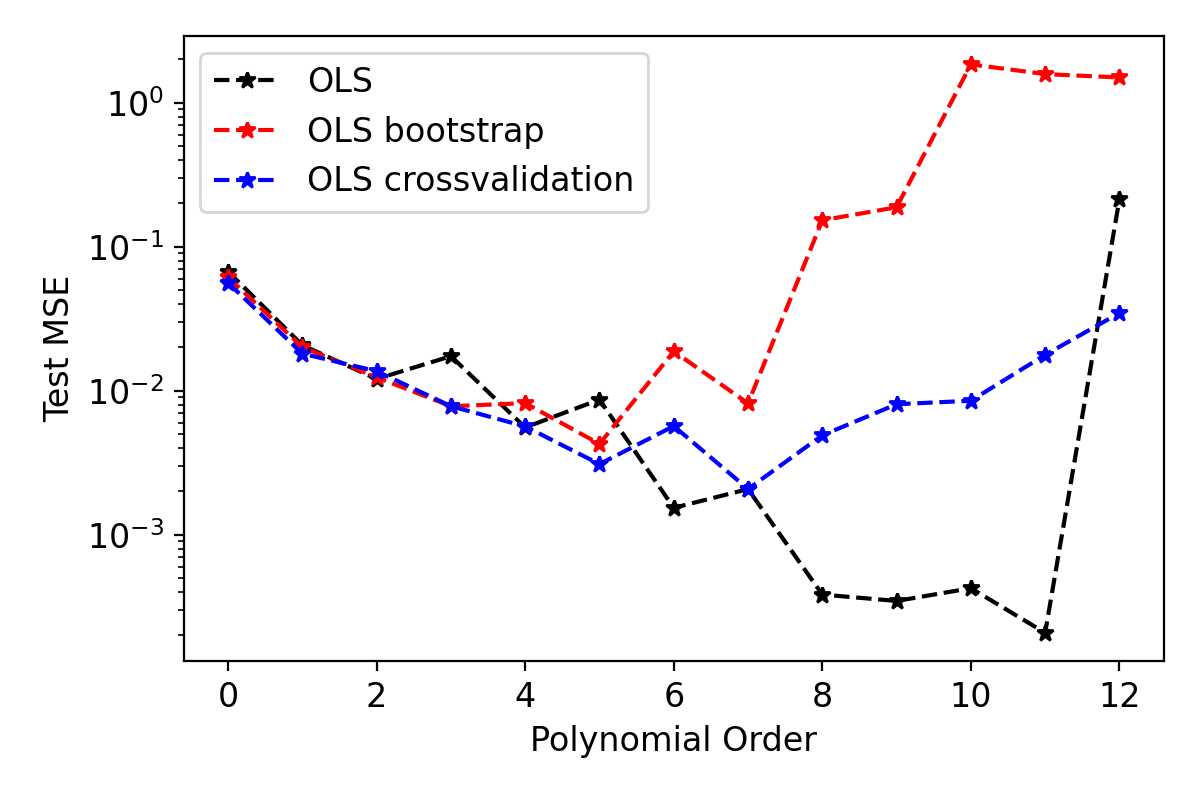
\includegraphics[width=.8\linewidth]{Images/ols14.png}
  \caption{}
  \label{fig:ols14}
\end{subfigure}
\caption{For $r=0.1$, $var=0$ and $n=100$: (a) $MSE_{train}$ and (b) $MSE_{test}$ plotted as functions of model complexity}
\label{fig:OLS_resample2}
\end{figure}

The figure \ref{fig:OLS_resample} shows the comparison between OLS, Ridge, and lasso methods with bootstrap and cross-validation resampling. Resampling is primarily performed to reduce the uncertainty in statistics like the mean squared error. Often, statistics of a single fit might not be the true indicator of the performance of the model due to the inherent stochasticity while splitting data into train and test sets, and in the noise. However, we see that in the case of OLS, the introduction of resampling has almost no effect. This can be attributed to the fact that due to $n = 900$, the model 'sees' a variety of data during the training phase. If the number of data points is reduced for example to $n=100$ (see figure \ref{fig:OLS_resample2}), then the effect of resampling is more prominent. We notice that for $n=100$, the training is equally well for OLS and OLS with cross-validation resampling. But, $MSE_{train}$ is lower for bootstrap for high values of $p$. This is an indicator of overfitting where, in bootstrap resampling, some of the data is 'seen' again due to sampling with replacement. This reduces the effective training set size and makes the model more prone to overfitting. This is also reflected in poor $MSE_{test}$ for OLS with bootstrap resampling. We also think that OLS with cross-validation resampling provides more reliable statistics than OLS without resampling as statistics of OLS with cross-validation can be thought of as a numerical average of statistics of multiple instances of OLS without resampling. The introduction of resampling in Ridge and lasso has no effect on training (figures \ref{fig:ridge9} and \ref{fig:lasso9}) but they do smoothen out the irregularities of the $MSE_{test}$ (figures \ref{fig:ridge8} and \ref{fig:lasso8}).


\subsubsection{OLS with Stochastic Gradient Descent}
For stochastic gradient descent (SGD) we have three additional parameters: the epoch $e$, learning rate $\eta$, and the number of mini-batches $n_{batch}$. See section \ref{subsec:SGD} for a detailed description of the SGD algorithm. The resource  \cite{masters_revisiting_2018} showed that using small batch sizes achieves the best training stability and test performance across a wide range of experiments. The best results were obtained for batch sizes equal to or smaller than 32. Therefore, we focus in this discussion on batch sizes 1, 2, 5, 10, 32. For a batch size of 1, we have a classical stochastic gradient descent. Otherwise, the algorithm is called mini-batch gradient descent. Usually, the number of epochs is large to sufficiently minimize the error by the learning algorithm. Therefore, we compare the output with epochs of size 10, 100, 500, 1000. Lastly, the learning rate is a small positive number and traditionally between 0 and 1. We analyze the output with the following learning rates 0.001, 0.01, 0.1, 1.0. \newline \newline
While the MSE for the training dataset hardly varies for different learn rates, number of epochs, or batch sizes the MSE for the test dataset improves slightly if the parameters are chosen correctly and the order of the fitted polynomial is high (see figure \ref{fig:ols_sgd}). The best results for $MSE_{test}$ were obtained for $n_{batch}=10, n_e=32$ and $\eta=0.1$. But even for the size of the mini-batches, which displays the "biggest" variance in the $MSE_{test}$, the difference is only between roughly $10^{-3}$ and $10^{-4}$ (see figure \ref{fig:olssg_test_batch}). To conclude, the choice of the SGD parameters, which we tested, does not seem to play an important part for the performance of the fitting in this case.

\begin{figure}[H]
\centering
\begin{subfigure}{.49\textwidth}
  \centering
  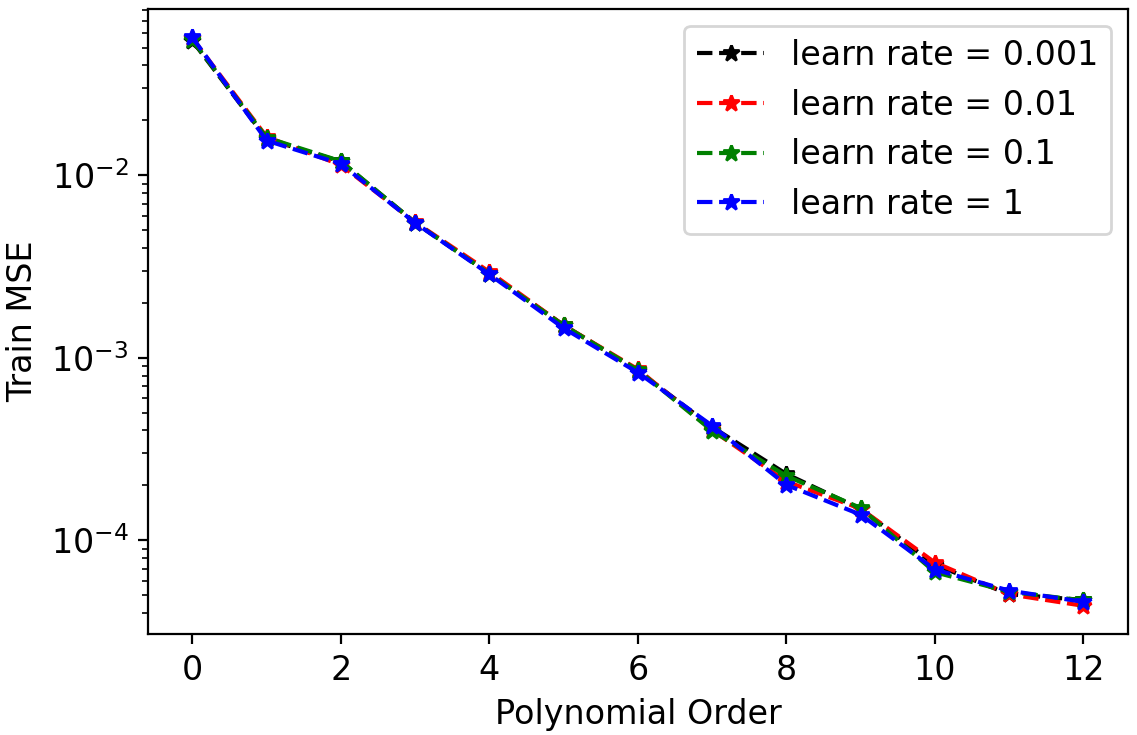
\includegraphics[width=.9\linewidth]{Images/olssgd_train_learn_rate_all_batch_32_epoch_10.png}
  \caption{}
  \label{fig:olssgd_train_learn_rate}
\end{subfigure}%
\begin{subfigure}{.49\textwidth}
  \centering
  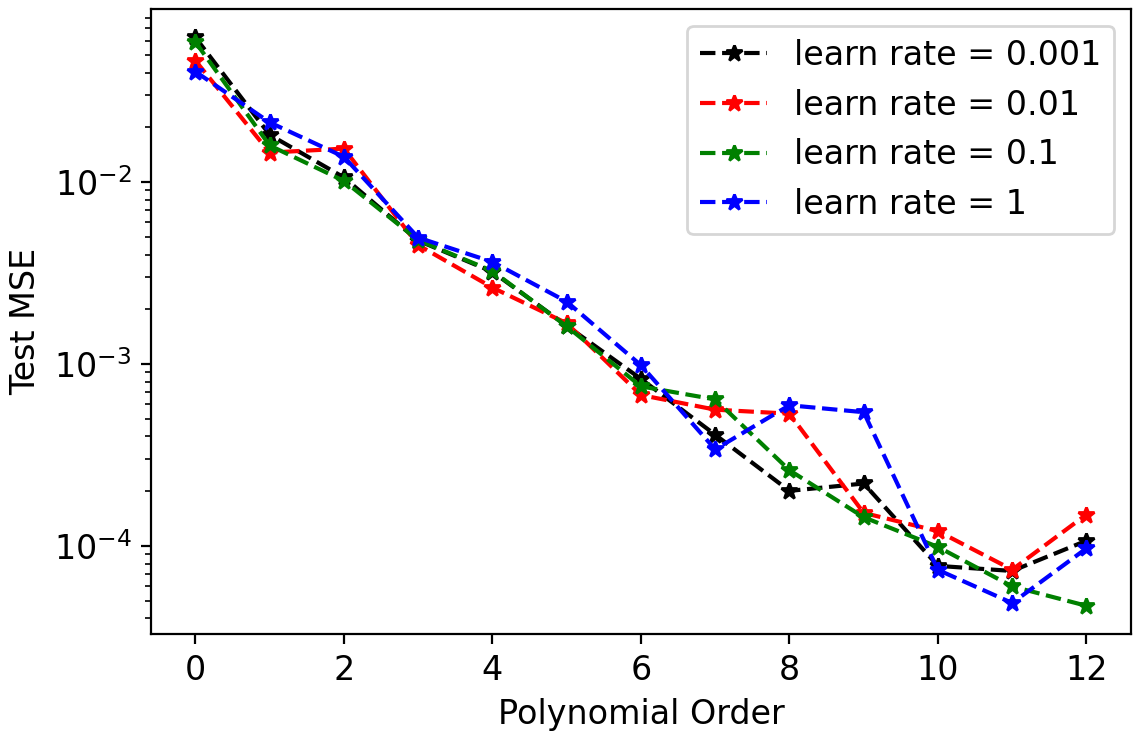
\includegraphics[width=.9\linewidth]{Images/olssgd_test_learn_rate_all_batch_32_epoch_10.png}
  \caption{}
  \label{fig:olssgd_test_learn_rate}
\end{subfigure}
\begin{subfigure}{.49\textwidth}
  \centering
  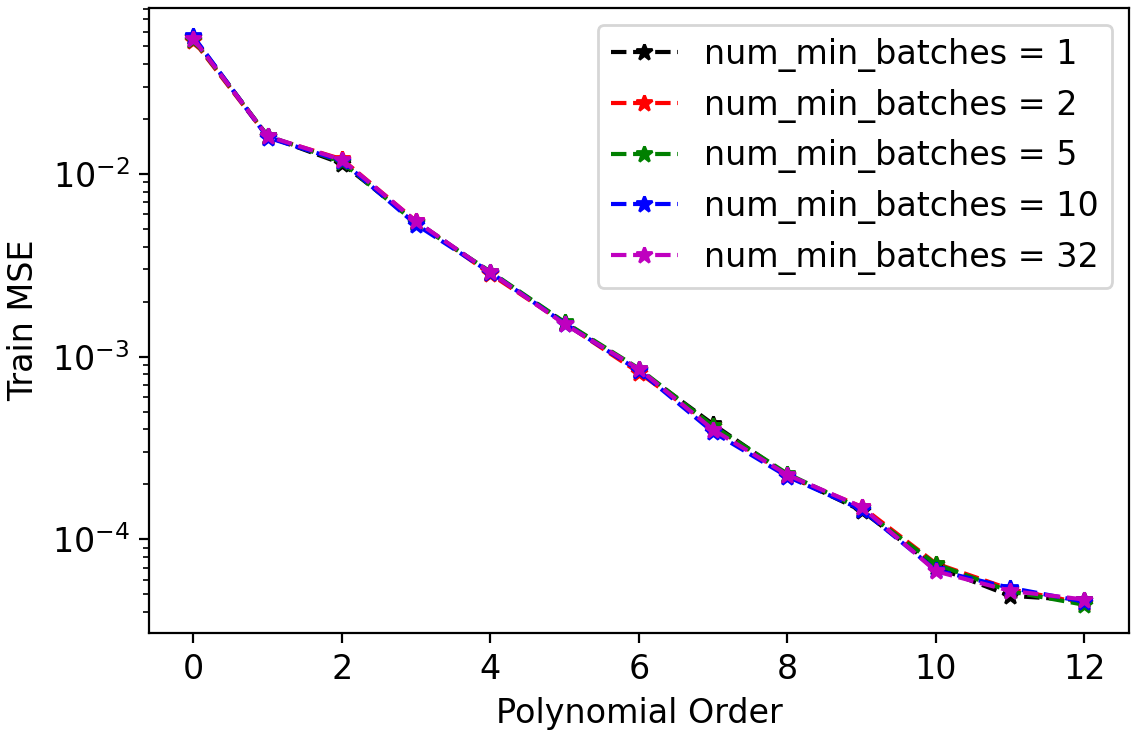
\includegraphics[width=.9\linewidth]{Images/olssgd_train_learn_rate_1_batch_all_epoch_10.png.png}
  \caption{}
  \label{fig:olssgd_train_batch}
\end{subfigure}
\begin{subfigure}{.49\textwidth}
  \centering
  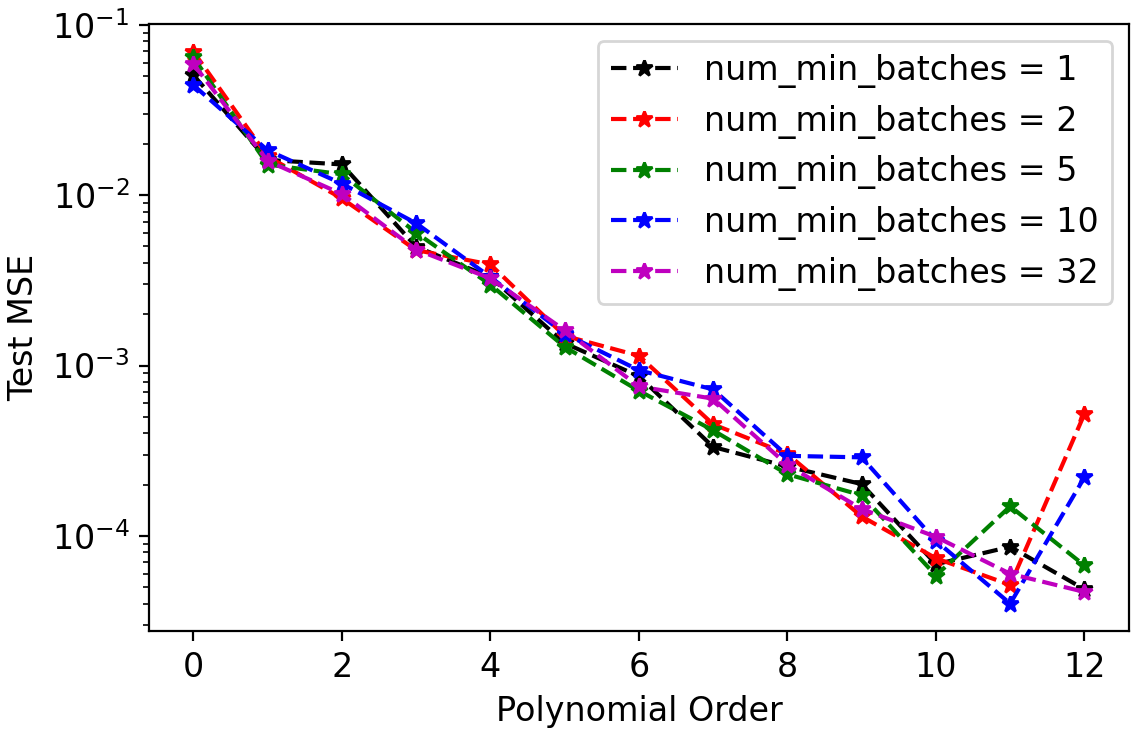
\includegraphics[width=.9\linewidth]{Images/olssgd_test_learn_rate_1_batch_all_epoch_10.png}
  \caption{}
  \label{fig:olssg_test_batch}
\end{subfigure}
\begin{subfigure}{.49\textwidth}
  \centering
  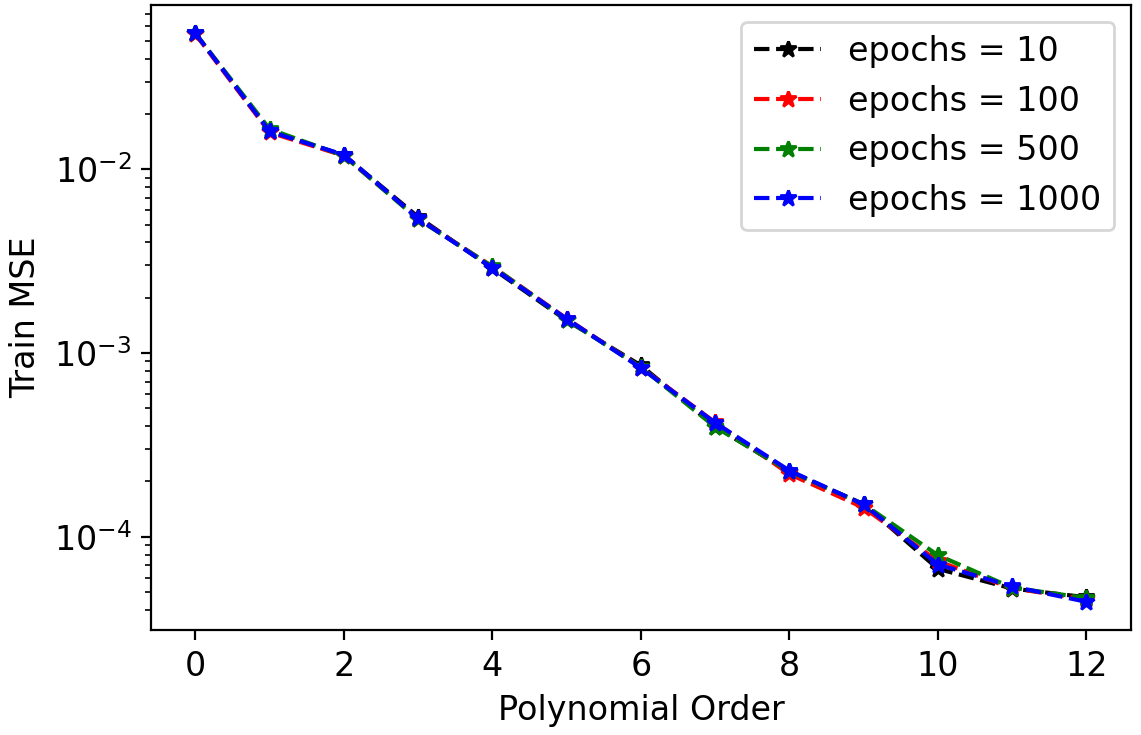
\includegraphics[width=.9\linewidth]{Images/olssgd_train_learn_rate_1_batch_32_epoch_all.png}
  \caption{}
  \label{fig:olssgd_train_epoch}
\end{subfigure}
\begin{subfigure}{.49\textwidth}
  \centering
  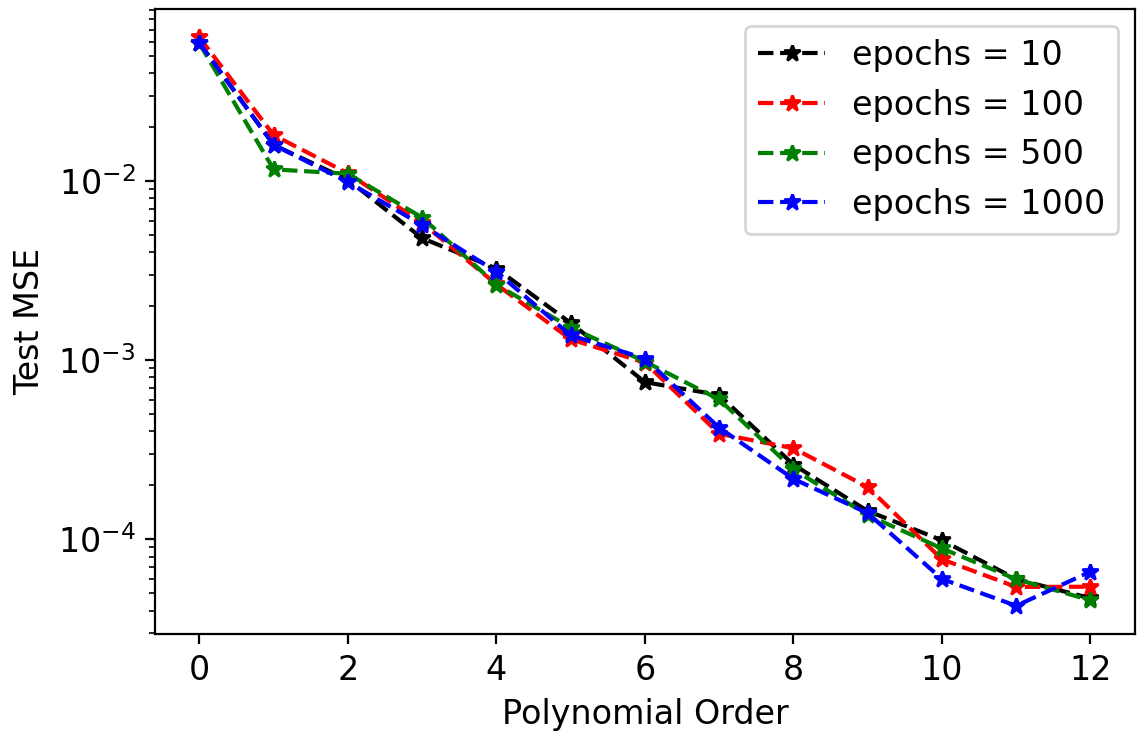
\includegraphics[width=.9\linewidth]{Images/olssgd_test_learn_rate_1_batch_32_epoch_all.png}
  \caption{}
  \label{fig:olssgd_test_epoch}
\end{subfigure}
\caption{For $r=0.1$, $var=0$, $n=900$: $MSE_{train}$ (left column) and $MSE_{test}$ (right column) plotted as functions of model complexity. a), b): $n_{batch}=10, n_e=32$, c), d): $\eta=0.1, n_e=10$, e), f): $\eta=0.1, n_{batch}=32$}
\label{fig:ols_sgd}
\end{figure}
Similar results were also obtained for optimizing the cost function for ridge regression. When we compare the test and train MSE for ridge and OLS regression with and without SGD (see figure \ref{fig:ols_sgd_ridge}) we clearly see that for OLS there is nearly no difference if the mini-batch stochastic gradient descent is applied or not. In contrary, when we look at ridge regression both the train and test MSE are better without applying the mini-batch stochastic gradient descent. For this simulation we used:  $n_{batch}=10, n_e=32, \eta=0.1$ and $\lambda_{ridge}=0.0001$. 
\begin{figure}[H]
	\centering
	\begin{subfigure}{.5\textwidth}
		\centering
		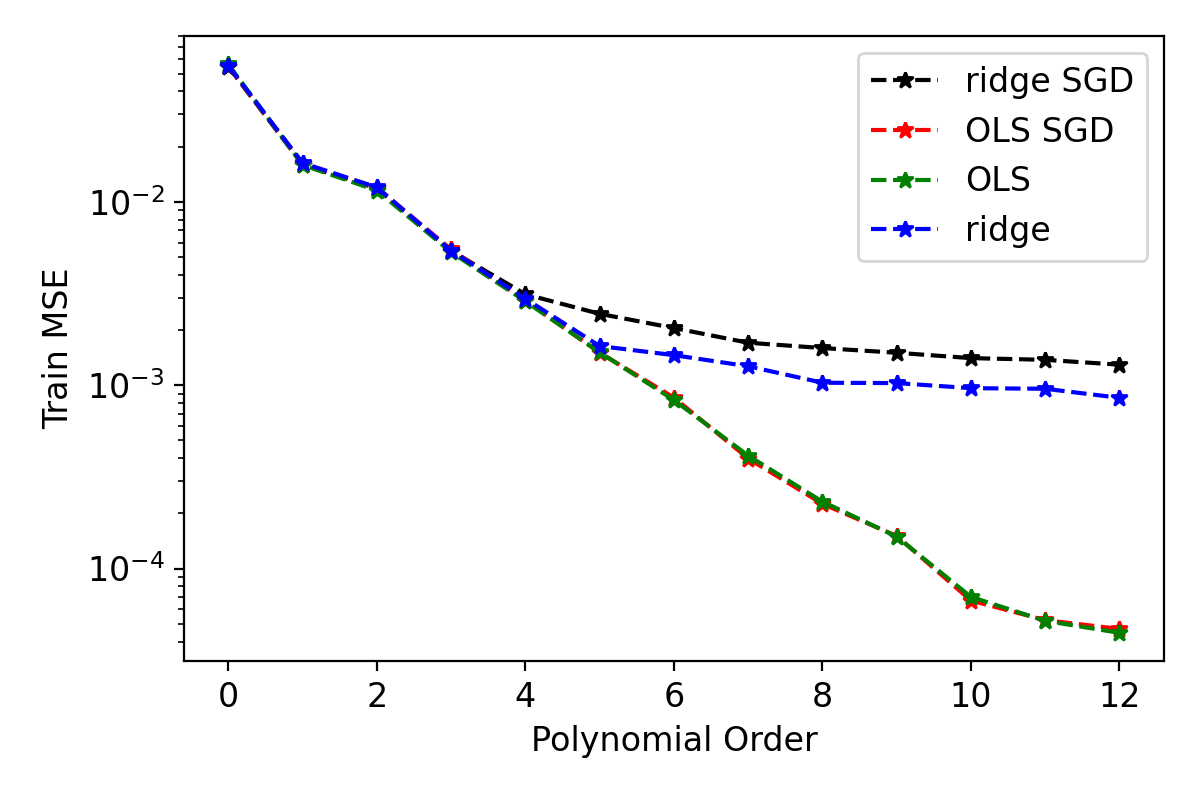
\includegraphics[width=.9\linewidth]{Images/sgd_ols_ridge_train.png}
		\caption{}
		\label{fig:ols_sgd_ridge_train}
	\end{subfigure}%
	\begin{subfigure}{.5\textwidth}
		\centering
		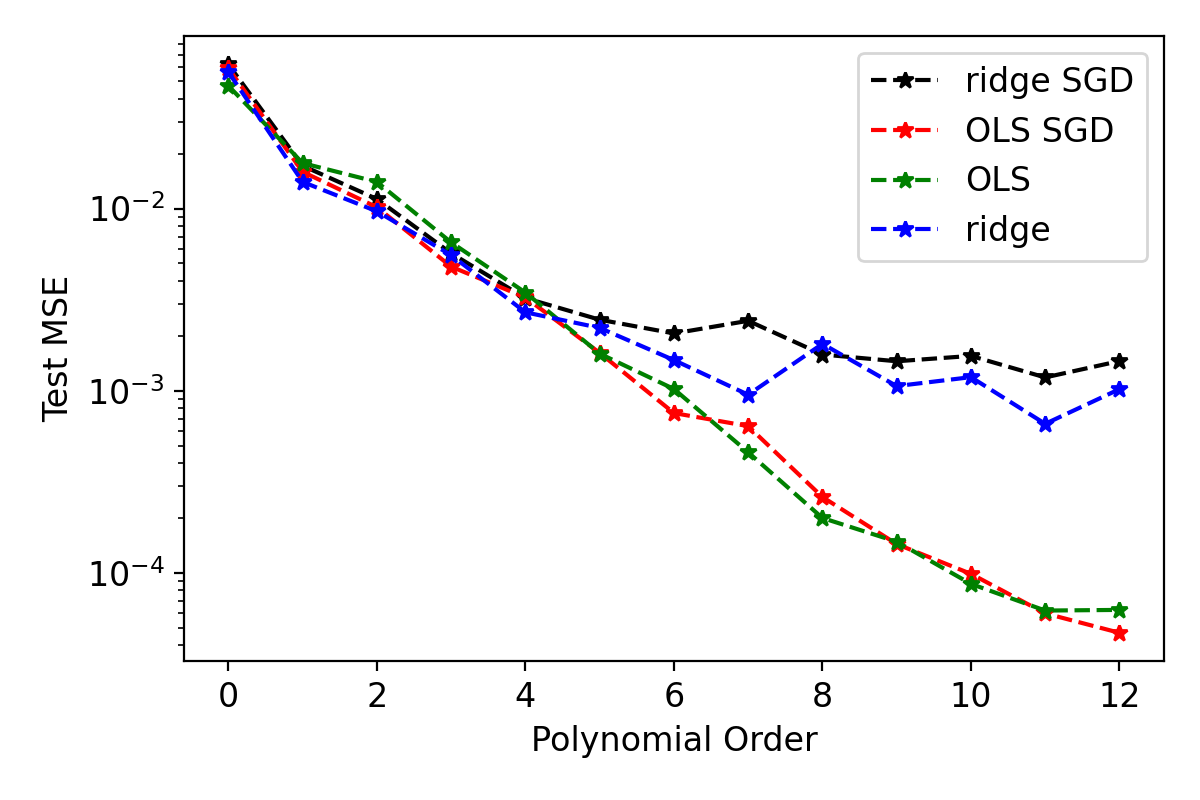
\includegraphics[width=.9\linewidth]{Images/sgd_ols_ridge_test.png}
		\caption{}
		\label{fig:ols_sgd_ridge_test}
	\end{subfigure}
	\caption{For $r=0.1$, $var=0$, $n=900$: $MSE_{train}$ and $MSE_{test}$ plotted as functions of model complexity.}
	\label{fig:ols_sgd_ridge}
\end{figure}